\documentclass[1opt,a4paper]{article}
\usepackage[utf8]{inputenc}
\usepackage[margin=1.5cm,includehead,includefoot]{geometry}
\usepackage[default]{lato}
\usepackage[T1]{fontenc}
\usepackage{multicol}
\usepackage{fancyhdr}
\usepackage{titlesec}
\usepackage{graphicx}
\usepackage{pdfpages}

\titlespacing{\subsection}{0em}{-0.1em}{-1.25em}
\titlespacing{\section}{0em}{0em}{0em}

%\titleformat{name=\subsection}
%{\normalfont\bfseries}{\thesubsection}{-1.25em}{}{}

\usepackage{url}
\usepackage{breakurl}
\def\UrlBreaks{\do\/\do-}

\usepackage{enumitem}
\setitemize{noitemsep,topsep=0pt,parsep=0pt,partopsep=0pt}
\setenumerate{noitemsep,topsep=0pt,parsep=0pt,partopsep=0pt}

\titleformat{\section}{\normalfont\Large\bfseries}{}{0em}{}
\titleformat{\subsection}{\normalfont\bfseries}{}{0em}{}

\pagestyle{fancy}
\fancyhf{}
\fancyhead[R]{\leftmark}
\fancyhead[L]{The Librarian}
\fancyfoot[C]{\thepage}

\renewcommand{\footrulewidth}{0.5pt}
\setlength{\headsep}{1.5em}

\setlength{\parindent}{0em}
\setlength{\parskip}{1.25em}

\newcounter{count}

\begin{document}

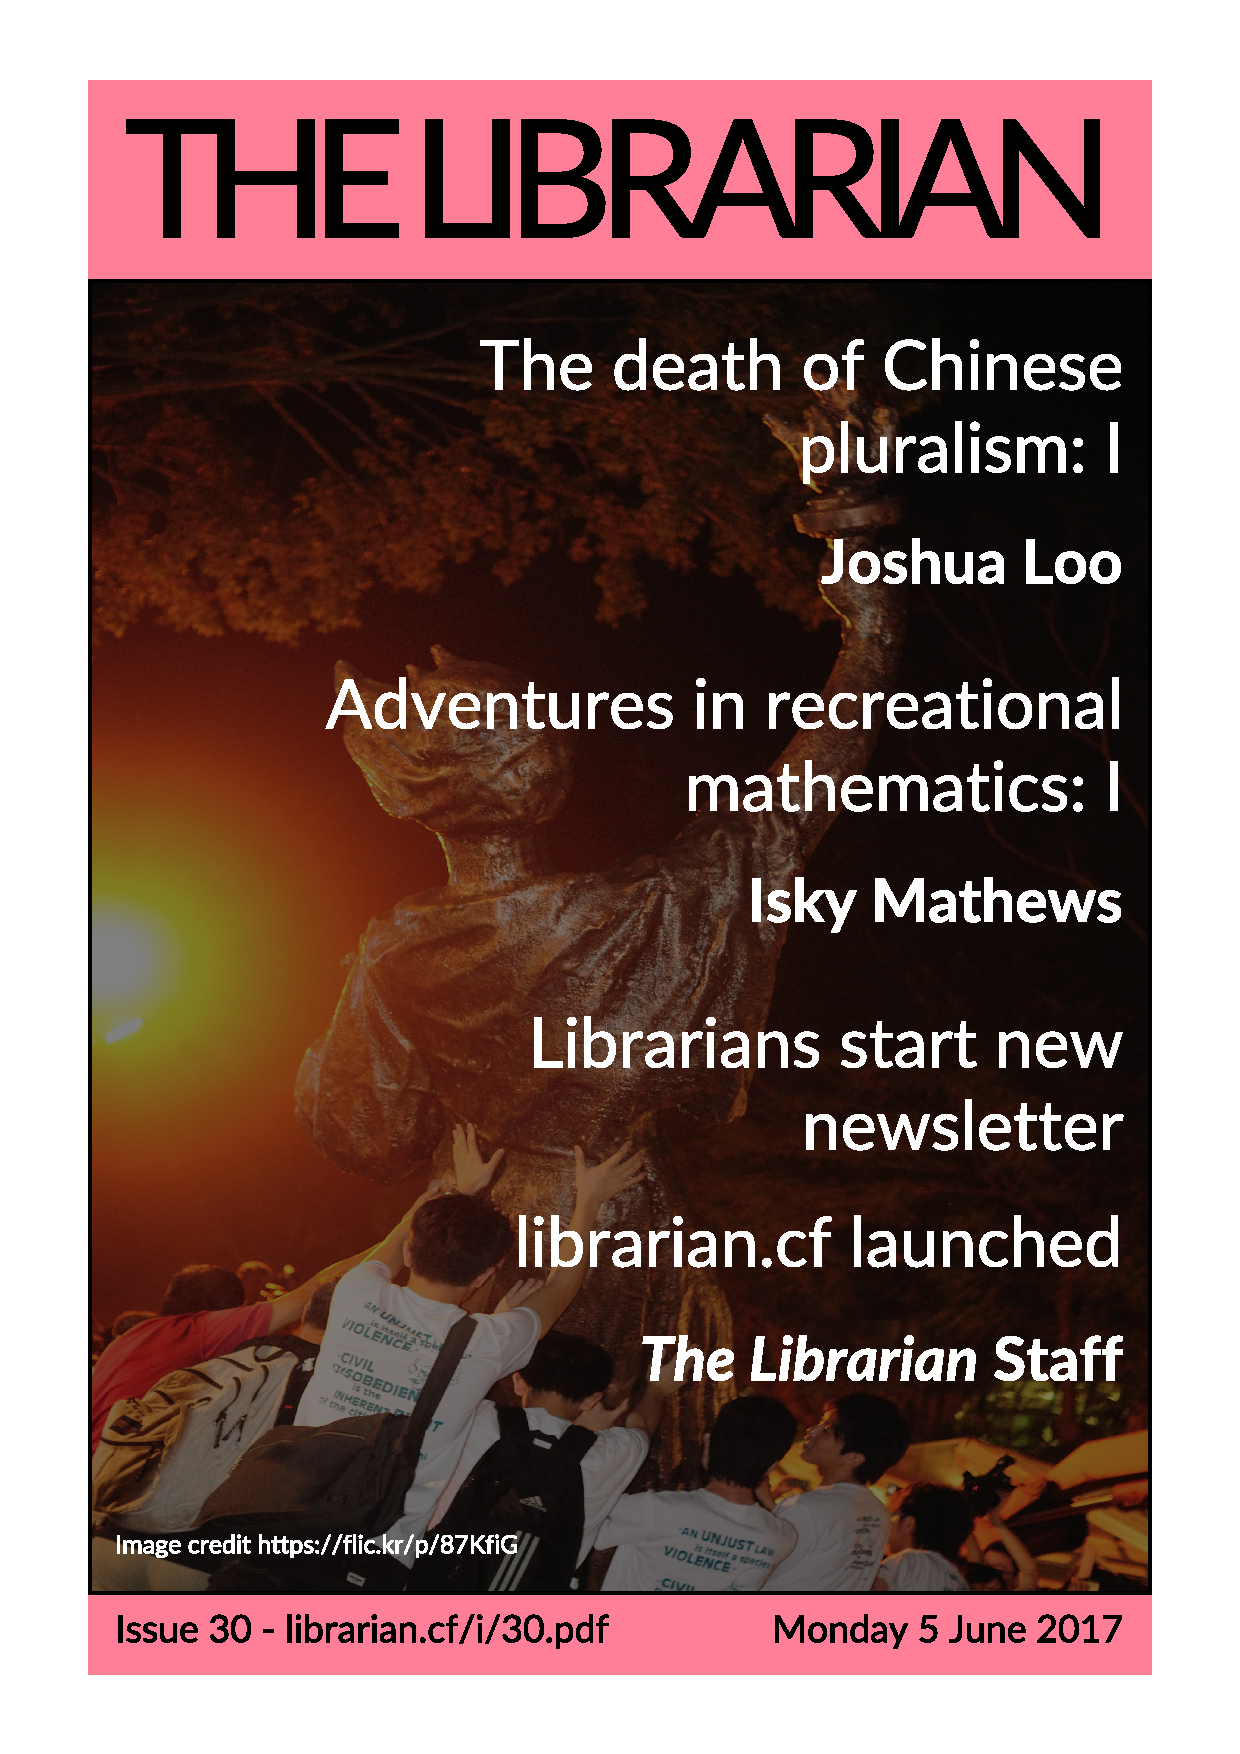
\includepdf[pages={1}]{30A4.pdf}

\section{Library News}
\begin{multicols}{2}
\subsection{The Librarian}
Agreement has been reached over editorial control of \textit{The Librarian}, confirming editorial independence and a new format of \textit{The Librarian}.

\textit{The Librarian} has also launched a website, available at \url{https://librarian.cf}.

A new one page summary of \textit{The Librarian} will be available from the water cooler within the next week.

\textit{The Librarian} is as usual open to submissions of articles. Isky Mathews and Ben Randall Shaw have started a new series \textit{Adventures in Recreational Mathematics}; Isky has kindly submitted the first article ready for this edition.\footnote{Please send articles to joshuapeterloo@gmail.com}

\subsection{Tinyletter}
Hear directly from the librarians about what they're reading and their work in the library at \url{https://tinyletter.com/wschoollibrary} - the last edition was published yesterday.

\end{multicols}

\section{Adventures in Recreational Mathematics: I}
\textbf{Isky Mathews}

\begin{multicols}{2}
Salutations!

This is the first of a new series in \emph{The Librarian }-- each issue,
we will discuss a different mathematical field or distinct problem
chosen due to their great utility, their results being intriguing or,
quite simply, their being enjoyable to play around with.

Each article will be written by one (or both) of \emph{Isky Mathews
and Benedict Randall Shaw}, discussing subjects we believe that others
will find stimulating as we do on a daily basis.

Also, for those interested, at the end of each article we will leave a
thematic problem of variable difficulty whose solutions should be
emailed to either one of the authors. Mathematics can be confusing, it
can be surprising but it can also be a lot of fun; this is what
\emph{Adventures in Recreational Mathematics} aims to tap into!

For our first issue, we will be considering \emph{tiling}. Tiling is the
study of how sets of polygons fit together on the plane, to see
whether they tile (i.e. can be placed together in such a way that
there are no gaps left across the plane) and to learn if there are
geometric principles which could allow us to determine whether these
sets can tile the plane or not. Formally, we are concerned with covering
the Euclidean plane formed by countable sets of \emph{closed sets} such that they intersect only on their boundaries. We begin with the
simplest form of tiling, \emph{regular} tessellation, where the tiling
is \emph{translationally similar} over arbitrary distances and uses only
identical regular polygons -- monohedral examples of this , which use only a single prototile, are very well known.

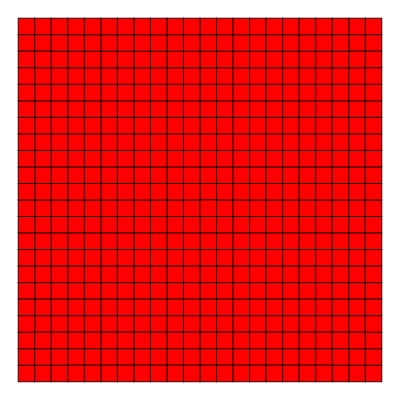
\includegraphics[width=\linewidth]{image_0.png}


\includegraphics[width=\linewidth]{image_1.png}


\includegraphics[width=\linewidth]{image_2.png}

We would also say that these tilings are \emph{isogonal }or
\emph{vertex-transitive, }i.e.~every vertex has an identical arrangement
of tiles around it, and also that they are \emph{edge-to-edge }tilings,
since a given edge of each tile touches no more than one edge from
another tile.

Perhaps unsurprisingly, it is trivial to prove that for \(∀ n∈R, n<2\)
there is an irregular \(n\)-gon which tessellates. This can be seen by
constructing the shapes below:

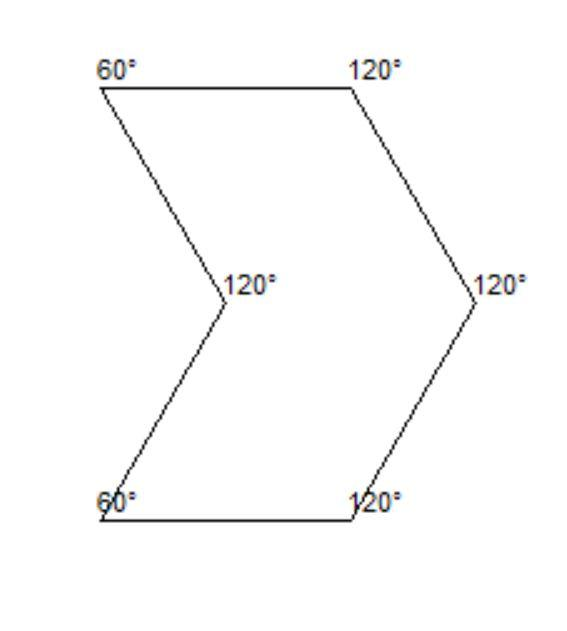
\includegraphics[width=\linewidth]{image_3.jpg}

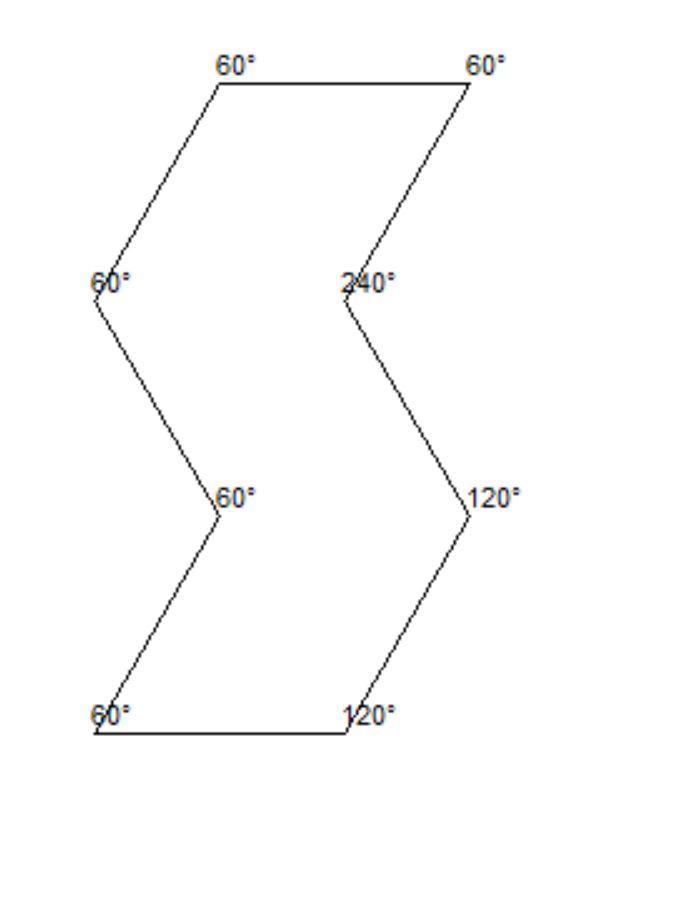
\includegraphics[width=\linewidth]{image_4.jpg}

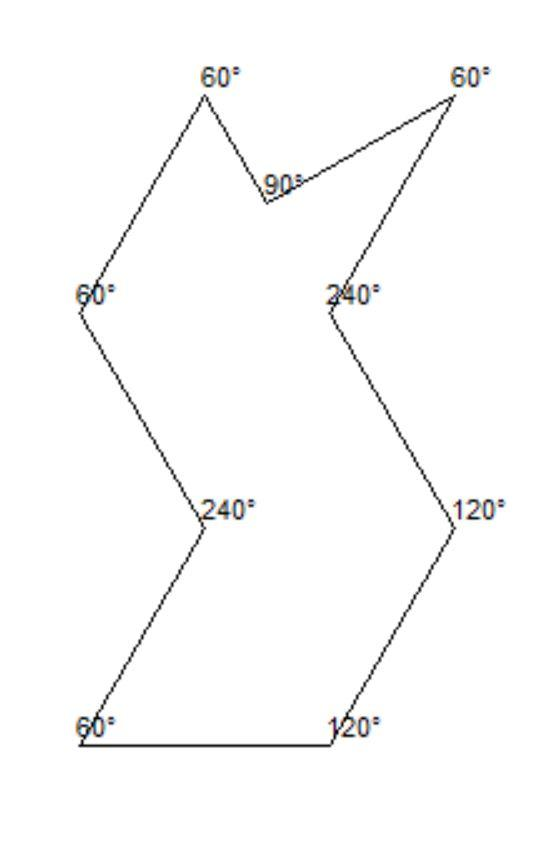
\includegraphics[width=\linewidth]{image_5.jpg}

The leftmost figure displays a tessellating hexagon and by adding
another pair of sides on top, we get the second figure (a tessellating
octagon). We can continue adding pairs like this to get tessellating
-gons for even. The third figure shows a way of making these figures odd
sided, while retaining tessellation (the forked parts can interlock with
two forked parts of other tiles). Thus, you can construct all even and
odd numbered polygons for using this method!

There are, as you can imagine, many other ways of constructing
tessellating -gons and in fact many ways of tiling them. If we allow
ourselves to tile on a plane with negative curvature (commonly
known as the \emph{hyperbolic plane}), then one can have significantly
more tilings -- for example, in the Euclidean plane we tile 6
equilateral triangles around a point but in the hyperbolic plane you can
have all the way to an infinite number of triangles around a point! This
geometry requires greater examination on its own, but that is not the
focus of the article.

There are also \emph{semiregular tilings}, those that are made up of
more than one tile but are still periodic, such as this lovely tiling
using squares, hexagons and dodecagons:

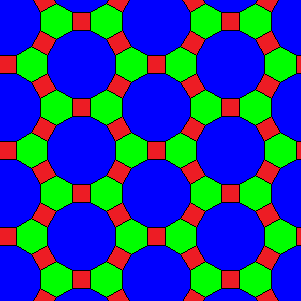
\includegraphics[width=\linewidth]{image_6.png}

However, these are all quite trivial examples and concepts. There are
numerous, seriously difficult problems: the so-called \emph{tiling
	problem, }the \emph{five-fold symmetry problem }and understanding
\emph{Heesch's Problem }are just a few.

The \emph{tiling problem} is to create an algorithm or set of principles
to determine whether a \emph{prototile set} tiles, in finite time. A
form of this was first proposed by the philosopher and mathematician Hao
Wang in 1961, after discovering sets of \emph{aperiodic} tiles called
\emph{Wang tiles. }An \emph{aperiodic tiling }is one that has no translational symmetry over any distance and \emph{aperiodic
	tiles }are those that can \emph{only }tile the plane aperiodically. The
colours on each side of a Wang tile are a visual way of representing
rules for placing them next to each other -- here only same-coloured
edges can touch but the same rules could just as easily be shown as
indents and projections on the edges of each tile. Due to these
``matching rules'', these tiles have become colloquially known as
\emph{Wang dominoes }and the problem of determining whether a set of
Wang tiles can tile the plane is often called the \emph{Domino Problem.}

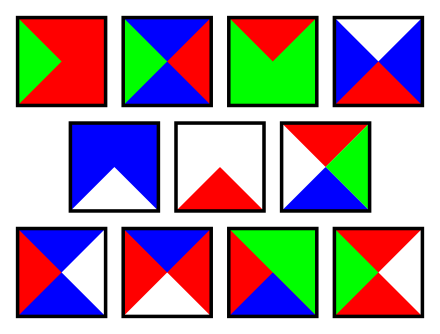
\includegraphics[width=\linewidth]{image_7.png}

In 1966, Wang's student \emph{Berger }showed that there is no
\emph{general }algorithm for the Domino Problem. More formally, he
showed that the problem is \emph{undecidable} by showing that it is
computationally \emph{isomorphic }to the \emph{halting problem }(the
first problem ever shown to be undecidable, by Turing). However, there
could be tiling-problem algorithms for subsets of the \emph{set of all
	tile sets }(for example, the Conway criterion) and some still search
for them today.

Heesch's Problem and \emph{Heesch numbers }were devised to help with the
creation of such an algorithm for single tiles and to give a
quantitative indication of the extent to which a tile does or doesn't
tessellate. The Heesch number of a tile is the maximum number of layers
of clones that can completely surround the previous layer's perimeter
and the eponymous problem is to determine precisely the set of numbers
that \emph{can be Heesch numbers. }To illustrate what this means,
consider a regular pentagon's Heesch number: 1.

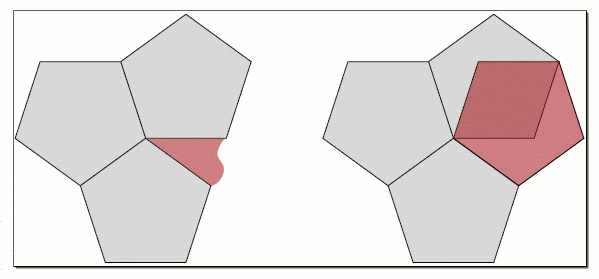
\includegraphics[width=\linewidth]{image_8.png}

This is because the 2nd layer would have to touch the sides inside the
cracks between the pentagons of the first layer (commonly referred to as
the first \emph{corona}), which is clearly impossible.

Can we have a tile of finite Heesch number? It appears so: in 1995,
Robert Ammann found a tile of Heesch number 3 and also constructed a
tile, using indentations and projections on sides of hexagons, of Heesch
number 4 and subsequently Casey Mann found an infinite family of tiles
of Heesch number \emph{5}, which is the highest finite number known to
date.

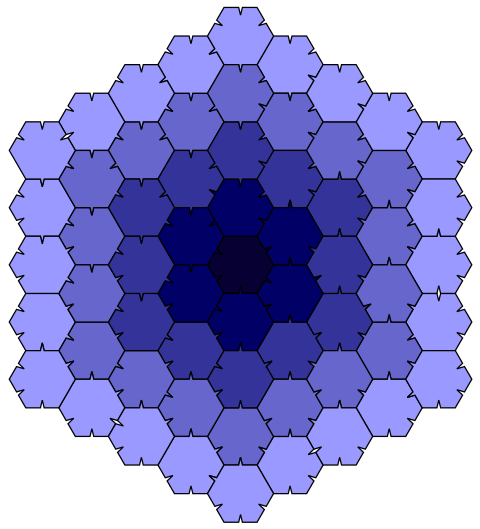
\includegraphics[width=\linewidth]{image_9.png}

You can see in the image that in the outermost layer there are four
cases where indents in the hexagons ``touch'' each other -- these parts
of the perimeter cannot be covered in the next layer, giving the
adjusted hexagon a Heesch number of 4.

The idea of the Heesch problem is to see whether there is a maximum
Heesch number . If this was true then you could construct a finite
tiling-problem algorithm: simply attempt to surround it by itself times
and if you can clearly continue then its Heesch number must be infinite,
thus proving that it tessellates. This algorithm wouldn't be
particularly efficient (at minimum, it would be an EXPTIME, potentially
even EXPTIME-complete, algorithm for those who are of the
\emph{computational complexity} persuasion) but it would represent a
great step forward.

This demonstrates one of the remarkable facts about tiling as a subject
to study: it is so simple to explain and to think about and yet its
problems are apparently so difficult. Beyond using rational thought,
having a good understanding of geometry and perhaps studying others'
work, there are no generally accepted tools or techniques used to solve
tiling problems. The majority of those who have moved the subject
forward have been individuals looking into the topic as a hobby.

If you've found this article interesting (or you just enjoy gazing at
beautiful tilings), we suggest these topics for further reading:

\begin{itemize}
	\item
	Roger Penrose's contribution to aperiodic tilings
	\item
	Wikipedia's wonderful catalog of \emph{Euclidean tilings by convex
		regular polygons}
	\item
	Golden Triangles
	\item
	\emph{The trouble with five }by Cambridge's \emph{Plus Magazine.}
	\item
	Voronoi tesselations
\end{itemize}

\subsection{Challenge I.:}\label{challenge-i.}

\begin{enumerate}
	\item The \emph{five-fold symmetry problem }is to find a tile set
	that consists of polygons with exactly five-fold symmetry or to show
	that such a set cannot exist. Your goal is much simpler, though themed
	on that basis: \textbf{Find one or more irregular pentagons that tile.}
	\item \textbf{Find a prototile/shape of Heesch number 3.} This is much
	harder, and we don't have the answer to this, so for the purposes of
	Westminster, this is an open problem!
\end{enumerate}



This article was written by \emph{Isky Mathews} but feel free to send
your solutions to either columnist!
\end{multicols}

\section{Reality \emph{may} not be what it seems: Lee Smolin's \emph{The Trouble With
		Physics}}

\begin{multicols}{2}

In 1905, Albert Einstein wrote three immensely influential papers: one
showing irrefutably the existence of the atom and its rough size, one
outlining Special Relativity and another introducing the concept of
\emph{energy quanta} to explain the photo-electric effect. Each of these
were so powerful not just because they solved long standing problems but
the implementation created \emph{testable predictions} of previously
unobserved phenomena and also brought great paradigm shifts
conceptually: General Relativity showed us that space's geometry was not
\emph{flat} and Quantum Theory demonstrated great abilities to predict
particle interactions and showed us that the universe is fundamentally
in some way probabilistic. It is the reconciliation of the last two
theories in a theory that once again brings new testable predictions and
new ideas to which Lee Smolin, a physicist currently working on quantum
gravity at the \emph{Perimeter Institute for Theoretical Physics},
devoted his 2006 book \emph{The Trouble With Physics.}

Quantum Theory and the models we have derived from it have been the most
successful physical theories ever: as Smolin points out, there have been
no experiments in the last 37 years which have done anything but confirm
the Standard Model of particle physics and if one discounts the
discovery that neutrinos have mass, a small but surprising revelation,
much longer than that. Smolin wrote his book worried that a whole
generation of physicists may have wasted their lives working on
something doomed to produce fewer and fewer meaningful results --
\emph{String Theory}. As he sees it, there are five great problems in
physics today:

\begin{enumerate}
	\item
	To combine General Relativity and Quantum Mechanics into a complete
	theory of nature. (the Problem of Quantum Gravity)
	\item
	To resolve the problems in the foundations of Quantum Mechanics,
	either by making sense of the theory as it stands or by inventing a
	new theory that does make sense.
	\item
	To determine whether the various particles and forces can be unified
	in a theory that explains them all as manifestations of a single,
	fundamental entity.
	\item
	To explain how the values of the free constants in the Standard Model
	of particle physics are chosen in nature.
	\item
	To explain dark matter and dark energy. Or, if they don't exist, to
	determine how and why gravity is modified on large scales. More
	generally, explain why the constants of the Standard Model of
	Cosmology, including dark energy, have the values that they do.
\end{enumerate}

Smolin states that back in the 1970s, when a few outcast physicists were
working on a succession to Kaluza-Klein Theory (the first attempt at
augmenting relativity to include electromagnetism) worked out that
mathematical objects called ``\emph{strings}'' can be made to propagate
using the simple law of minimising area, leading to quantised
frequencies at which they vibrate. These frequencies were found to
correspond with the particles in the Standard Model (even originally the
graviton featured as a \emph{gravity-carrying boson}), changing such
individuals as \emph{Edward Witten} from obscurity into the physics
world's celebrities. This already solved one of the five problems stated
above and potentially had something to say about quantum gravity but as
the theory was studied in more depth, serious and cavernous problems
became apparent.

In this book, Smolin takes you through the history of the world's most
studied physics theory, from the First Superstring Revolution to Edward
Witten's conference conjecture of M-Theory to the great Maldacena
Conjecture. He shows clearly why something which he and a generation of
others once had so much faith in has failed to live up to its creators'
expectations and why perhaps it is tentative now to even call it a
theory, as there are no generally accepted proposals about what the main
principles of the theory are nor what the main equations are, nor any
proof that they could exist.

In fact, the problem, as he demonstrates, may be far deeper than String
Theory but rather in the \emph{celebrity culture} it breeds, a
tremendously self-confident establishment with an unusually monolithic
community which members describe in terms similar to religion and seem
to agree on myriad concepts with a strong sense of consensus whether
driven by the evidence or not. More than a revision of theory but a
revision of the structure of the entire theoretical physics field may be
necessary.

\emph{The Trouble with Physics} is a book for those truly keen on
theoretical physics but despite their best efforts, have yet to
understand all the mathematics. Despite never showing a single equation,
Smolin goes into great depth on the web of concepts and it partners very
well with other books in the genre, such as Carlo Rovelli's
\emph{Reality Is Not What It Seems} and Penrose's \emph{Faith, Fashion
	and Fantasy in the new physics of the Modern Age}, truly showing you
where they brush dirt under the carpet and explain things overly
optimistically. Smolin applies the ultimate sceptical lens, critiquing
everything, even his own work and life. He admits that he was a String
Theorist for some time but during his university years, he says ``my
friends and I would never have guessed that we were living through the
last days of theoretical physics as we knew it.''

If you're particularly intrigued from a technical perspective, the book
contains explanations of: branes and strings, the Maldacena conjecture,
M-Theory, S-Duality and other dualities, gauge theories, Doubly Special
Relativity, spontaneous symmetry breaking, supersymmetry, the
Hawking-Entropy Paradox, Kaluza-Klein Theory, Loop Quantum Gravity and
much more. Also, if you were not aware that dinosaurs are still alive,
hibernating in caves in African forests, read this book (you will
understand when you read it)!

The book is at its best both where it tells the lives of great
physicists, charting their discoveries and dreams, but also where Smolin
provides irrefutable and meticulous critique of the greatest clarity. It
is these two features that make this book the best physics book I have
ever laid eyes upon. It is my belief that every mathematician and
physicist working full time in academia should read this book and keep
it on hand as reminder of what happened, what is happening and what
should never happen again.
\end{multicols}

\section{The Death of Chinese Pluralism: I}
\textbf{Joshua Loo}

\begin{multicols}{2}

About 100 thousand Hong Kong residents marked June 4 with an annual commemoration of the Tiananmen Square massacre. These commemorations provide an important reminder of the true nature of the Chinese state. They are important on their own, by virtue of the sheer barbarity involved in the massacre. Yet they now are perhaps important for us in a self-interested calculus.

China matters. Almost everyone acknowledges now that it matters, and that whatever rhetoric surrounds its rise is not wholly ``hype'', as it might have been of Japan. It matters not only in the UK, where $7\%$ of our electricity supply will soon be reliant on Chinese goodwill and engineering\cite{hinkley}, in Africa, where China has built vast quantities of infrastructure including railways and roads with a pledge of \$60bn of investment\cite{ifrica}, or in those parts of the Eurasian landmass which are to be connected by its One Belt One Road initiative, but also in the entire world with universal and undeniable force, when the vast majority of the computing equipment essential to the working of the modern world is manufactured in China.

When such a rise occurs, it is important that the nature of the rising power is analysed, both out of an intrinsic need to know of one's fate as interaction with China changes both in intensity and in balance and out of a need to make informed choices as to those dimensions in interaction with China.

First, three initial examples will help to illustrate the scope and aim of this article.

Yang Shuping, a student at the University of Maryland, said in a graduation speech that she felt the "fresh air of free speech" during her time at university\cite{yang}. Ordinarily, this would not be a particularly incisive or controversial idea. Though the United States may be suffering from slippage in freedom of speech, the free exchange of ideas is in much better shape in the United States than in China\cite{press}\cite{freedomhouse}. When the video was posted on Weibo, a group of Chinese students posted a video titled ``\#Proud of China UMD", whose prologue claimed that the commencement speech contained "false statements and rumor [sic] about multiple China-related issues. We are deeply concerned about some of the stereotypical comments in her speech."\cite{umd} Apart from some embellishment in relation to air pollution in her city of Kunming, it's not clear exactly what was taken issue with.

``We need to open up and embrace all the suggestions from outside world," claims the first speaker. "I would be so piss[ed] off if anyone described my country with destruction\footnote{The audio isn't entirely clear.}," she continues.

A few days before, China held a ``Belt and Road initiative" meeting in Beijing. One notable absence was that of Lee Hsien Loong, Prime Minister of Singapore; Singaporean media speculated that this was due to an incident several months prior, wherein a Terrex armed vehicle was impounded by Hong Kong authorities while returning from a training exercise in Taiwan\cite{beltroad}.

Several months earlier, a mainland legal expert proposed an adjustment in the ratio of foreign judges in Hong Kong, after a foreign judge, David Dufton, sentenced police officers who assaulted protestors in the 2014 Occupy Hong Kong protests to jail\cite{foreignjudge}.

Although all these incidents appear to be unrelated, they are a symptom of a deeper maliaise which touches the heart of every state and establishment, but does so with particularly problematic consequences in states which have experienced recent political ruptures or are lack conventional accountability mechanisms. China, which suffers acutely from both problems, is run by a leadership both in great need and with few sources of legitimacy.

These travails may seem to be the unimportant rumblings of a faraway Eastern nation. They are not. They will soon, if they do not already, affect you and me as much as they affected Yang and Dufton. When China was introverted, it was easy enough for its political oppression to stay within China; now that it has opened up, it is willing and able to exert pressure on outside actors to change their behaviour, often for the worse. It is therefore important to question what motivates the Chinese state and how it comes to decisions, in order to determine what is likely to occur as a result of this externally as well as internally.

This article will explore the ways in which the Chinese state can achieve legitimacy. It concludes that, in the absence of democratic reform, the Chinese state will either collapse or become increasingly stridently nationalist, associating Chinese identity with so-called ``Chinese values'' of dictatorship and international dominance, which presents a number of problems for other states, both in their treatment of Chinese citizens and in their relations with China.

\subsection{The foundations of the Chinese nation state}

On 12 February 1912, millennia of tradition in the world’s longest continuously surviving civilisation came to a halt, as the child Emperor abdicated. An interregnum marked by instability, military domination by warlords and misery ceased upon communist victory on 1 October. Outwardly, the revolution took the form of a comprehensive movement away from ideals which dated back to the preceding millennium. This was, too, the case inwardly. Between 750,000 and 1,500,000 million were killed in a campaign of mass and popular depravity\cite{puyi_autobio}.

The democratic aspirations of the Chinese people may have been illusory, limited merely to Western-connected intellectuals. Yet 12 February marked also a time in which the Chinese people threw off the shackles of imperial authority. The speed of change is striking. Nominally one of the world’s most powerful people in 1912, Puyi, the child-emperor of China in the last days of empire, spent a decade in Communist prison camps before retiring to write a pro-Mao memoir-cum-apologia, in which he wrote ``I covered up my crimes in order to protect myself”\cite{cultural_revolution}, in reference to his justifications for cooperation with the Japanese in Manchuria.

Inwardly, however, one pressure remained - the need for legitimacy. The removal of millennia of institutional inertia presented the greatest opportunity for democratic renewal that China has ever faced. Although democratic systems occasionally suffer from legitimacy problems due to low turnout, inherent in democratically elected governments is at least some degree of popular support, and so there is a floor of legitimacy. Dictatorships' floor of legitimacy is such that they only are overthrown when a sufficient proportion of the people feel so incensed by regime incompetence or manevolence that they attempt to overthrow the government.

First, we must ask ourselves where legitimacy is derived from, particularly in a Chinese context.

China is not entirely alien to the rest of the world. Its people care about life, liberty (in a sort of collective sense, although perhaps not individually) and other basic needs. In this sense, Chinese regimes need, like other regimes, to ensure that people living under them are adequately fed, housed and clothed. The failure of the republican leadership to do this during the civil war can be said to have lead to their downfall, because it encouraged support for the communists. This need, however, is not absolute. Many Chinese dynasties limped on while their people languished in poverty, and the communists themselves. In that sense, legitimacy derived from living standards exists in China as it exists universally.

There are also ideological concerns and ways of achieving legitimacy. For thousands of years, the idea of the Mandate of Heaven created loyalty to the emperor, at its basic heart. However, it was sufficiently flexible to allow new emperors or dynasties to take over, when ``Heaven'' decided that the emperor or a dynasty had become too venal and corrupt to deserve its mandate. In this way, it provided a useful tool by which to, somewhat external to material concerns, rule. As a result of its great and increasing age, it managed to survive for thousands of years as the basis of Chinese government; we conclude from this that it was quite successful in its aim. 

The Mandate of Heaven is not the only way by which ideological legitimacy can be created. The communists attempted to replace this with a utopian vision of a Maoist society. The degree to which this was successful is quite difficult to ascertain. On the one hand, there was great enthusiasm in the campaign against ``intellectuals'' and other undesirables during the Cultural Revolution and Great Leap Forward. On the other hand, those same people who probably were around persecuting unfortunates quickly reversed their stance and displayed great flexibility in adapting to first ``Socialism with Chinese characteristics'' and then its true face, ie. some form of state capitalism, with all the rent-making opportunities that implied. Were all these hundreds of millions of people really genuinely convinced that Mao was a great visionary who had all the answers, but simultaneously able to adjust? Or, as is more likely, were they moulded by circumstance, perhaps to some degree motivated by genuine fervour, but really largely simulated by each other? One shout to ``kill 1000 intellectuals'' would likely have been followed by another hundred in a sort of collective inaction problem - what if one is the next to be deemed a reactionary for insufficient revolutionary fervour?

How does this apply to the new regime? First, any new state will have problems in finding popular legitimacy. This is inevitable when revolution necessarily causes all the old institutions of government to, at the very least, lose power or fragment. As a result, many basic services which citizens rely on the government to provide and/or would expect of any government, including at the very least security, are likely not to be provided. This problem was compounded by a deliberate policy of repression of ``intellectuals'', ie. people who had a university education or vaguely had knowledge of how to run things which China needed, like power stations or transportation networks. Given this, the foundation of the Chinese state was not built on material concerns - indeed, it had to be actively shifted away from such concerns because initial administration was so poor.

Second, the Chinese state was deprived of the idea of the Mandate of Heaven. Not only were they not monarchical, which meant that such ideas were already largely impossible, given that the Mandate of Heaven was given to an emperor and his/her descendants, collectively comprising a dynasty, they were also diametrically opposed to the intellectual fabric which gave credence to such ideas, in that they sought to destroy traditionalist ideas of God, religion and emperor. We can therefore discount divine legitimacy as a source of inspiration.

Third, what is left is pure ideology. The sole mechanism by which the communists were able to gain legitimacy was ideological struggle, a mechanism which is hard to sustain in this solitary manner. Not only would it have, at some point, come into conflict with the necessity of preventing state collapse - legitimacy is a mechanism to stay in power, but if external factors mean that even with perceived legitimacy one collapses, it does not help, a reliance on ideological struggle fails because of its inherent idealism, which is incompatible with practical problems causing a failure to achieve utopia.

Precipitately, the foundations upon which the Chinese state were built were entirely precarious, and especially ill-suited to China.

\subsection{Normalisation}

This situation could not go on, and it did not. Many will be familiar with at least an outline of what happened under Deng Xiaoping. Economic liberalisation, and a decision to cease the continual shooting-oneself-in-the-foot policies which marked Maoism, meant that the state could refocus itself on achieving the first type of legitimacy, ie. that based on material concerns.

This worked, for a while. China lifted 800 million people out of poverty and is now the largest economy in purchasing power terms in the world. Yet 10\% growth is barely sustainable. China has been growing at this rate for nearly four decades. It cannot continue for much longer - growth is now down to below 7\%, and may fall further. Independent sources of information which might tell us without government interference what the real economic situation is in China, but until then we are dependent on the government for such information.

The Chinese leadership, however, recognises that it is very difficult to continue to use ideological fervour to sustain the legitimacy it has created based on economic growth. This puts it in a very dangerous situation, because the measure needed to ensure long term growth and hence long term stability are in conflict with measures which would simulate the economy in the short term in order to stave off loss of legitimacy.

It is difficult to determine whether this is true. Government approval ratings in China are often above 90\%, but even if they are conducted impartially, it is possible and indeed quite likely in a nation which went through the trauma of the Cultural Revolution that these polls are affected by culturally ingrained reminders to toe the party line, both because it is correct in an objective sense, and because such toeing is in one's self-interest.

More easily, one can analyse the measures that the Chinese government is taking to ensure that it retains control. This, as a first step, indicates that it is worried about its control of the country.

\subsection{Increasing dictatorship}

Liberalisation, and democratic stagnation/reversal, in China, largely took place on three tracks: first, internal party mechanisms of control, second, information control, and third, other civil liberties like freedom of movement and freedom from torture.

After the excesses of Mao, the communists in China recognised that they too would have to face up to the ``bad emperor problem'': with a high level of state control, one can enrich oneself and the country with good policymaking, but should a bad ``emperor'' or ``paramount leader'' as the case may be come to power, the whole of China would face severe difficulties. Mao was their ``bad emperor'', and he taught the communists the virtue of true collective leadership. Although the communists have not become paragons of liberal or democratic virtue, it is notable that the infighting which characterised the Party under Mao significantly abated under the mechanism of collective leadership. The solution of collective leadership works by slowing down the acquisition and exercise of power by its diffusion. In doing so, one has fewer ``bad emperors'', even though progress is slowed. It is indubitably superior to the days of Mao or Stalin, and is superior in that it prevents massive shifts in Party power from one faction to another in the hope of achieving total poewr - instead one vies for positions within the Party and the individual powers they offer.

As for information, after Mao, it was significantly freed up. This reached its peak under Zhao Ziyang, but still remained better throughout all of China than under Mao. Chinese media report on a number of social and environmental issues, including smog, contamination from industrial pollutants, and local government incompetence. Although this coverage is often scaled back or retrospectively deleted after censors become nervous, the Chinese people still remember articles after they are deleted. Similarly, somewhat liberal academics were, to some degree, free to debate, within their universities and their dormitories, with less government interference, compared with Mao-era detention and expulsion to the countryside of all academics. In mnay cases, this lead to a degree of introspection which was not present in Mao-era China. This provided great potential for a gradual and optimised transition to democracy and accountability, for it would not have occurred in a vacuum of knowledge.

It cannot be pretended that China was at any point a state which respected certain basic rights of its citizens, like their bodily autonomy or property rights. At no point did the culture of state impunity which pervaded instituions like the ``People's Armed Police'' abate significantly - they were still free to oppress the people. However, what did change was that they were used less. There was less state violence post-Mao. Fewer properties were seized. Torture was used less, and in some cases the judiciary even admitted that it was wrong. This was real progress - certainly not enough for those who still are victimised by it, but still real.

The 18th National Congress of the Communist Party of China marked the start of a turning point in this slow movement towards democratic legitimacy. It initially appeared to be the start of faster movement. Corruption trials of senior party officials finally went ahead. Chinese officials didn't stop mourners from flocking to the house of Zhao Ziyang, a reformist, to mourn his death. Xi was a new face, representing a new era.

These illusions soon wore off. The corruption trials were really a tool to achieve greater power within the Communist party for Xi and his friends. Indeed, Xi himself is said to be suspiciously wealthy, and he and his family hold a number of properties outside China. Chinese officials probably didn't mind letting people mourn Zhao Ziyang because very few people remember him and they felt that their hold on power was greater than ever before, with their control of the main means of transmission of information, ie. the internet. When people posted pro-Zhao messages on internet message boards, they were deleted, but their posters were not rounded up and detained.

Perhaps a new face, Xi is most certainly not doing anything other than shoring up the dictatorial powers of the party.

Xi has been named the ``Core of the Party'', and many commentators suggest that he has more power than any leader since Deng Xiaoping. Some have even suggested that he may wish to continue after his customary pair of five year terms in positions in the Central Military Commission and Party, though he may resign as President as is constitutionally mandated. In his attempts to corral the paty into submission, it is feared that he may have alienated so many officials that the only way to ensure that he is not arrested just as he has arrested some former officials is to stay in power, and that means that we must wait until his death, not his retirement, to see the back of him.

Information controls have been re-imposed. Liberal academics find themselves under increasing pressures to make universities conform as a tool for communism. No longer are the authorities content to leave them as bastions of ineffective and bourgeois liberalism, never seriously mounting a challenge to Communist leadership - they want them to actively participate in their programme of brainwashing the people.

Repression continues unabated. Dissidents are denied access to their lawyers. An environmental documentary which observers initially thought would be permitted under a new censorship policy of tolerating environmental polemics was soon prohibited. Lawyers of dissidents are occasionally detained. Sometimes their lawyers are detained. The state appoints its own lawyers for them, who are often incompetent and fail to defend them at all - the reason why should be obvious.

This is already bad. It indicates that the government of the most populous government in the world does not even pay lip service to ideals of human dignity and accountability, and that anyone who even suggests it ought to runs the risk of finding their lives turned upside down. Actual observance of these norms is out of the question. But it is also normal. Lots of governments have acted like this, and their peoples have still managed to recover to some degree. Many dictatorships have also ruled over large numbers of people. Part I is a reminder that a powerful nation is increasingly at odds with the values which not only the West but much of the world holds dear. Part II of this series will explore the ways in which China is spreading its influence across the world, and why China therefore presents a problem perhaps unprecedented in the history of humanity in its propagation of its own values, if they even exist as such and are not simply base interests.
\bibliographystyle{unsrt}
\bibliography{citations.bib}

\end{multicols}

\includepdf[pages={2}]{30A4.pdf}

\end{document}
